

\section{Data Management Organization Structure}
This section defines the organization structure for the period in which the DM System is developed and commissioned, up to the start of LSST Observatory operations.  Refer to chapter 6 for Pre-Construction Phase Organization.
The DM Project Manager and DM Project Scientist, who are known collectively as DM Management, lead the DMO.  The Project Manager has direct responsibility for coordination with the overall LSST Project Office, the LSST Change Control Board, the LSST Corporation, and LSST partner organizations on all budgetary, schedule, and resource matters.  The Project Scientist has primary scientific and technical responsibility in the DMO and responsibility for ensuring that the scientific requirements of the LSST are supported, and is a member on the LSST Project Science Team (PST). 
As shown in \figref{fig:dmorg}, the organization now features lead institutions, each with responsibility for major element of the DM System (Level 2 Work Breakdown Structure elements).  For example, during Final Design, the Process Control and Archive Site Manager and Team at NCSA will be conducting prototyping activities in computing, data communications, and data storage to select and verify the ability of System technologies to support the LSST requirements.  They will also be involved in creating a supporting infrastructure for the DM Systems.  During Construction before the LSST first light time frame, these resources will be focused on implementation of the selected technologies.  In order to ensure that team functions as one integrated project, the institutions coordinate support by other lead institution team members directly through this organizational structure, as well as via a number of cross-organizational bodies (described later in this document). 
Also, due to the span of the organization, the DM Project Manager may be supported by one of the lead institution Project Managers as a Deputy Project Manager in these phases.

\begin{figure}[htbp]
\begin{center}
 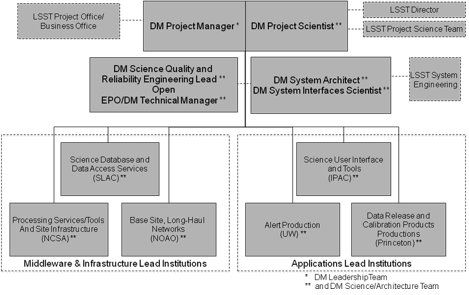
\includegraphics[width=0.9\textwidth]{images/dmorg}
\caption{Example Product tree a version of  CU1 product tree \label{fig:dmorg}}
\end{center}
\end{figure}

\section{Data Management Cross-Organizational Control Bodies}
Since the DM team is distributed in terms of geography and responsibility across the LSST partner and lead institutions, mechanisms are needed to ensure that the project remains on track at all times.  There are three primary coordinating bodies to ensure the management, technical, and quality integrity of the DM project.  All DM institutions have membership on these bodies, and all meet at least once per month during construction and commissioning.
\subsection{DM Leadership Team}

The DM Leadership Team (DMLT) purpose is to establish scope of work and resource allocation across DM and ensure overall project management integrity across DM.
The following mandate established the DMLT:

\begin{itemize}
\item Charter/purpose
	\begin{itemize}
	\item Establish scope of work and resource allocation across DM
	\item Ensure overall project management integrity across DM
	\item Ensure Earned Value management requirements are met
	\end{itemize}
\item Membership
	\begin{itemize}
	\item Co-Chaired by the DM Project Manager, (TBD DM Deputy Project Manager(s)
	\item Core members are Lead Institution Technical/Control Account Managers (T/CAMs or CAMs)
	\end{itemize}
\item Responsibilities
	\begin{itemize}
	\item Prepares all budgets, schedules, plans
	\item Meets every week to track progress, address issues/risks, adjust work assignments and schedules, and disseminate/discuss general PM communications
	\item Creates and publishes monthly, quarterly, annual progress reports
	\item Meets at start of each software development phase with SAT to establish detailed scope/work plan
	\item Meets with SAT for change control (TCT)
	\end{itemize}
\end{itemize}

The DM Leadership Team and the Science/Architecture Team (SAT) work in synchrony. The SAT (and the various DM team members as delegated) is responsible for creating, establishing, updating, analyzing, proposing the reference and DC designs and changes to them, whether they might affect the DMS requirements, the reference design, or the Data Challenges. The DMLT makes sure the requirements and architecture/design are estimated and scheduled in accordance with LSST Project required budgets and schedules.
\subsection{Science/ Architecture Team}

The Data Management Science/Architecture Team (SAT) is chaired by the Data Management System Architect and Project Scientist. The SAT is the DM-wide body that is charged with addressing issues of the overall requirements flowdown, architecture, and organization of the design of Data Management, both for the final LSST design and for the Data Challenges.

The designs and other high-level outputs of the SAT become part of the technical baselines for Data Management in the LSST project and for the Data Challenges. Approval and change control for these baselines are managed by the DM Technical Control Team (TCT).

\begin{itemize}
\item Charter/Purpose
	\begin{itemize}
	\item Support DM System Architect in ensuring that the DMS meets science requirements
	\item Support DM Project Scientist in ensuring DMS has overall scientific integrity
	\item Control all DMS internal and external interfaces
	\item Perform or delegate due diligence for proposed technical baseline changes; then recommend changes (or no action) to the TCT
	\item Decide issues involving internal, non-change-controlled DM architecture and design
	\end{itemize}
\item Membership
	\begin{itemize}
	\item Co-Chaired by the DM System Architect (Kian-Tat Lim), DM Project Scientist (Mario Juric)
	\item Core Members are Institutional Scientific/Technical Leads
	\end{itemize}
\item Responsibilities
	\begin{itemize}
	\item Meets at start of each software development phase with DMLT to establish detailed scope/work plan
	\item Meets with DMLT for change control (TCT)
	\item Supports the System Architect's role in the systems engineering process, notably in the establishment and review of interface requirements and Interface Control Documents with the other LSST subsystems
	\item Conducts (or delegates) design reviews and code reviews during the LSST development process
	\item Endeavors to instill a productive and ethical engineering culture within DM
	\item Commissions Working Groups
		\begin{itemize}
		\item Working groups are architectural (e.g. Applications, Middleware, Database, Infrastructure, Operations), span subsystems
		\item Chaired by a member of the Science/Architecture Team
		\item Members include other technical personnel, possibly including outside collaborators
		\end{itemize}
	\end{itemize}
\end{itemize}

\subsection{Technical Control Team}
The DM Technical Control Team has responsibility for issues similar to those of the LSST Configuration Control Board, but restricted to those contained within the DM subsystem. The TCT reviews and approves changes to all baselines in the LSST Data Management System, including proposed changes to the DM System Requirements' (DMSR), reference design, sizing model, i.e. any LDM-xxx baselined document.  The TCT makes sure these changes don't get into the baseline without proper change control.  Note that the TCT does not author the Technical Baseline and has no specific technical deliverable charter, but it does validate that the form and content of the Technical Baseline is consistent with LSST project standards such as the System Engineering Management Plan (SEMP).  Specific responsibilities for development of the Technical Baseline and evaluation of the content versus LSST and DM requirements are elsewhere in this document.
\begin{itemize}
\item Charter/purpose
	\begin{itemize}
	\item Ensure that the DM Technical Baseline (LDM-xxx) documents are baselined and once baselined only changed when necessary, according to LSST and DM configuration control processes
	\end{itemize}
\item Membership
	\begin{itemize}
	\item Co-Chaired by the DM Project Manager and DM Project Scientist
	\item Members include the DM System Architect, DM System Interfaces Scientist, DM SQuaRE Technical Manager
	\item For on-line virtual meetings, if a quorum is not reached within one week, the DM Project Manager and the DM Project Scientist will make a unilateral decision
	\end{itemize}
\item Responsibilities
	\begin{itemize}
	\item Determines when specification and deliverables are of sufficient maturity and quality to be baselined (placed under configuration controlled status) or released. The TCT reviews and approves proposed changes to baselined items.
	\item Reviews and approves/rejects proposed changes to baselined items
	\end{itemize}
\end{itemize}

